\section{Introduction}

As the level of phylogenetic analysis increases---from individual
loci, to chromosomes, to genomes containing multiple chromosomes---so
too does the computational complexity. In \poy, a significant
increase in computational time results from combining cladogram
searching with co-optimization of nucleotide pairwise alignments,
rearrangements of loci within a chromosome, and rearrangements of
chromosome fragments within the genome.  As a result, a phylogenetic
analysis involves a set of nested computationally ``hard'' (NP-complete)
problems that makes finding exact solutions extremely unlikely. In
addition, increasing sequence length heterogeneity (at the levels
of nucleotides, loci, and chromosomes) and the ever-growing sizes
of datasets, further contribute to computational complexity.

To cope with the problem of computational intractability, and
hence, the speed of the analyses, \poy can employ a battery of
approximate, or heuristic methods that function at different levels
of the analysis. As with all heuristic procedures, a tradeoff is
involved: a substantial decrease in execution time comes at a price
of obtaining solutions with reduced optimality (however, the extent
of the tradeoff is difficult to evaluate in the analyses of real
datasets). Therefore, it becomes important to understand the combined
effect of different heuristic methods, so that the chosen search
strategy balances the computational time with a ``reasonable''
quality of the result.

Here, we provide general guidelines for using different heuristic
methods, exploring their combined effect, and suggesting the choice
of parameters that can be explored to provide the best result for
specific cases. Real datasets differ greatly in size and complexity,
so that no single optimal strategy can be suggested. These guidelines,
however, should enable the investigator to design an efficient
strategy that can be tailored to the peculiarities of a given
dataset.

In addition to heuristic methods, this chapter attempts to assist
with the selection of transformation cost regimes.  Alternative
cost regimes can significantly affect the outcome of the analysis,
this becomes particularly apparent in dealing with large, genome-level
datasets, where multiple cost regimes are used simultaneously to
specify transformations at different levels of analysis. Many
problems stem from the difficulty in selecting the most reasonable
combination of parameters for the optimization of DNA sequence data
at the levels of nucleotides, loci, and chromosomes.

\section{Preparing data files for analysis}
If molecular sequence files contain incomplete sequences, it is {\bf highly}
recommended that the file be partitioned prior to analysis in \poy.
Partitioning or fragmenting the data can help to ameliorate the effects of
poor sequences, missing data, or the lack of overlap of sequences---as
is very often the case when incorporating sequences that were downloaded 
from an online database such as GenBank (as different studies may have 
utilized different priming regions) (Figure~\ref{fig:primer_chop}).

At the level of nucleotides, individual fragments in a locus can
be separated by pound symbols (``\#'') or contained in individual
files (that is, treated as partitions). When ``\#'s'' are used,
their number must be the same across homologous sequences.
Alternatively, the argument of \poyargument{auto\_sequence\_partition}
of the command \ccross{transform} can partition the data. This
command evaluates each fragment in the data file and if a long
region appears to have no indels, then the fragment is broken inside
that region. \poyargument{auto\_sequence\_partition} works best
when primer flanking regions are available. When primer flanking 
regions are not available it is recommended that 
the ``\#''s be inserted manually (Figure~\ref{fig:messyseq_prechop} and 
Figure~\ref{fig:messyseq_postchop}).

\begin{figure}[htpb!]
\begin{center}
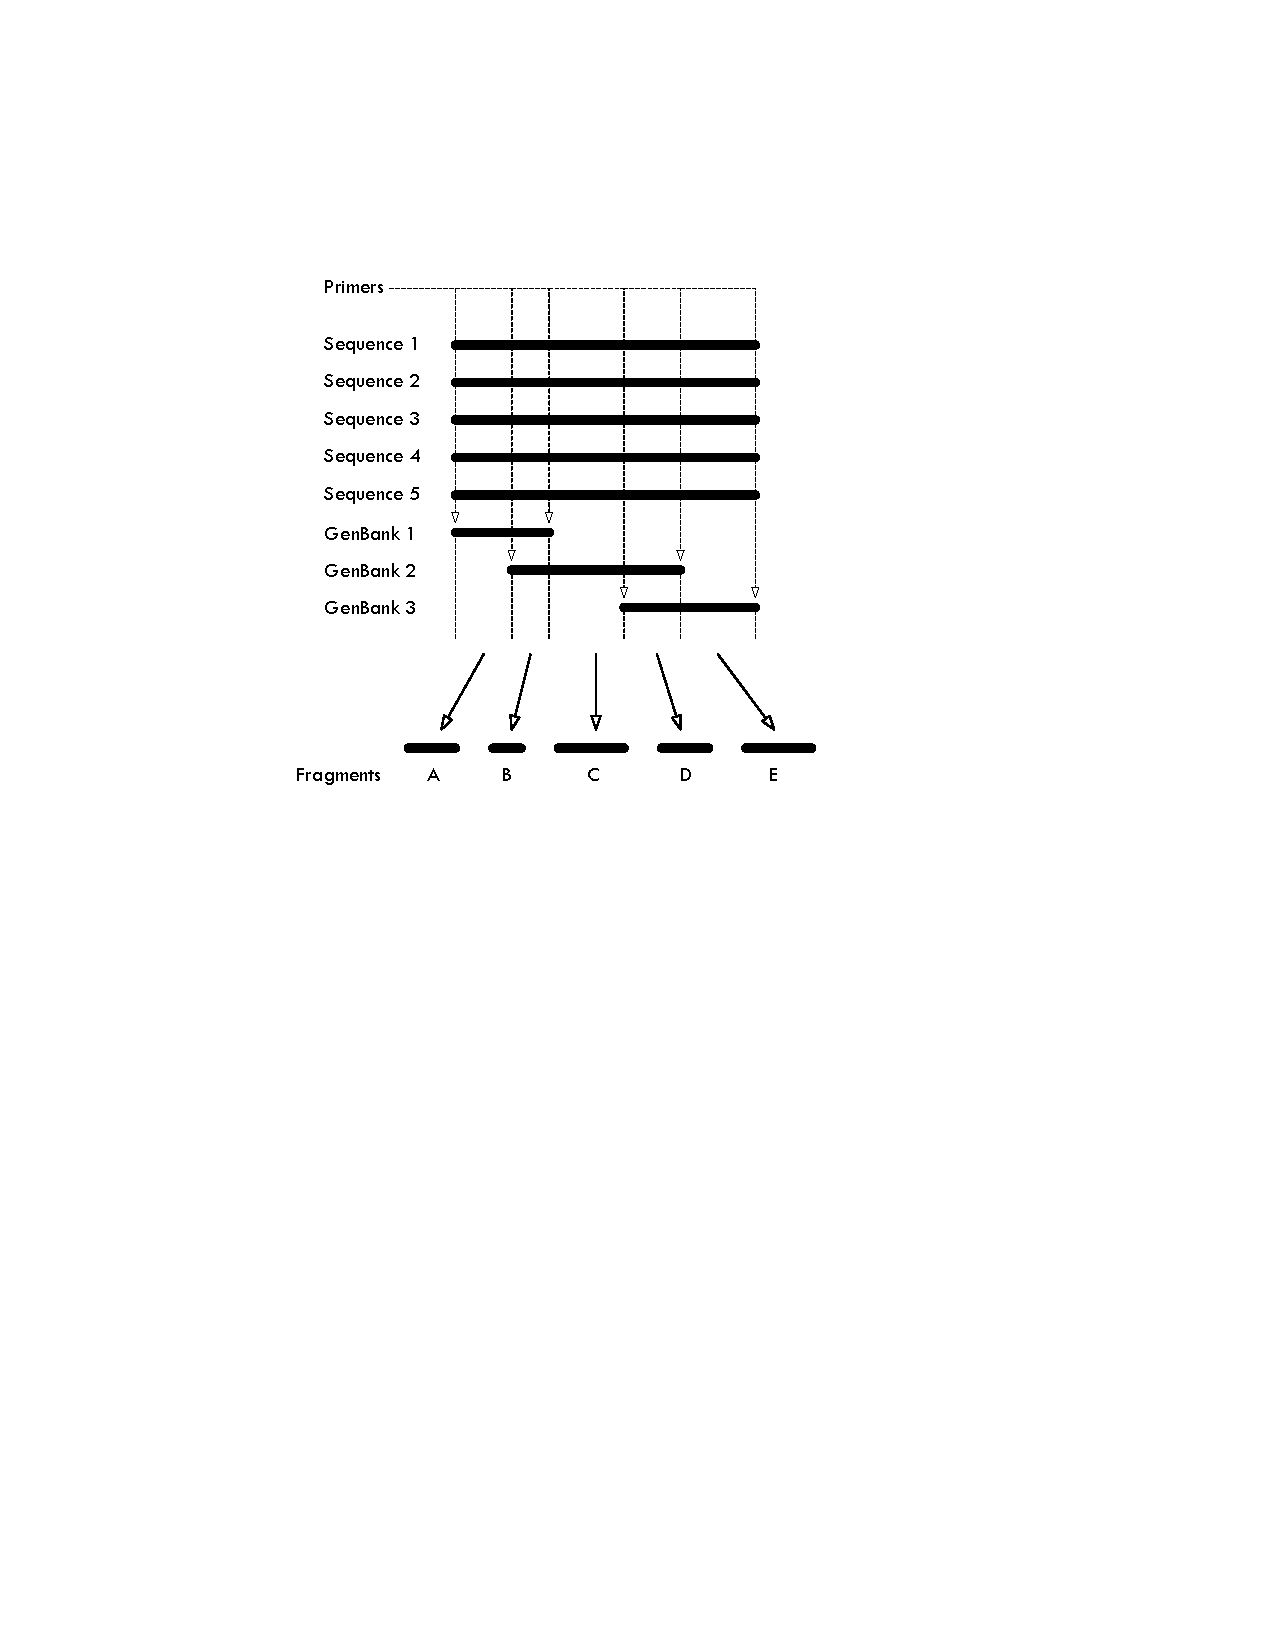
\includegraphics[width=0.75\textwidth]{doc/figures/primer_chop.pdf}
\end{center}
\caption{Separation of eight sequences into fragments, using flanking primers 
as a guide.  This partitioning will help to ameliorate the effects of missing data in the
sequences \texttt{GenBank1}, \texttt{GenBank2}, and \texttt{GenBank3}.}
\label{fig:primer_chop}
\end{figure}



\begin{figure}[htpb!]
\begin{center}
\includegraphics[width=1.0\textwidth]{doc/figures/messyseq_prechop.pdf}
\end{center}
\caption{A nucleotide sequence alignment visualized in BioEdit.}
\label{fig:messyseq_prechop}
\end{figure}

\begin{figure}[htpb!]
\begin{center}
\includegraphics[width=1.0\textwidth]{doc/figures/messyseq_postchop.pdf}
\end{center}
\caption{A nucleotide sequence alignment visualized in BioEdit, that has been 
`chopped', via insertion of ``\#'' symbols. ``Cnemaspis\_limi'' and 
``Phyllopezus\_pollicaris'' have been modified with the insertion of N's.
Note the lack of overlap between ``Delma\_tincta'' and ``Phelsuma\_lineata''.}
\label{fig:messyseq_postchop}
\end{figure}


\section{Data treatment}

Direct optimization (see \emph{Character optimization} section
below) involves comparing potential nucleotide homologies between
two sequences. Consequently, the time it takes is proportional to
the product of the lengths of the sequences compared 
($O(n^2)$)~\cite{wheeler2012book}. 
This procedure can be time consuming for
long sequences and for those DNA fragments that greatly differ
in length. In cases where unambiguous (such as long, completely
conserved regions) sequence fragments can be identified, partitioning
the long sequences into smaller fragments delimited by these regions
can significantly reduce computational time. Such economy is reached
because nucleotide homologies are not examined over the separate
partitions. This strategy assumes that the fragments are mutually
exclusive and are homologous across terminals.

\begin{table}[!t] 
\small
\caption{Heuristics Guide: Data Treatment.}
\label{HeuristicsGuide1} 
\begin{center}
\renewcommand{\arraystretch}{1.5}
\begin{tabular}{p{2.5cm}  p{3.4cm}  p{5.4cm} } 
\hline
	Level of analysis & Heuristic & Implementation \\
\hline
	Nucleotides and amino acids  & Fragment sequences & Manually separate fragments with \# symbols or transformed using
	\poycommand{auto\_sequence\_partition}\\
	Locus & Fragment chromosome & Manually insert pipes (``$\vert$'') separating loci \\
	Chromosomes & N/A & N/A \\
\hline
\end{tabular}
\end{center}
\end{table}

As mentioned previously, nucleotide sequences can be  partitioned 
by inserting pound symbols (``\#'').  Fragmenting long sequences greatly accelerates searching.
At the chromosome level, individual loci can be separated by pipes
(``$\vert$'') (see Table \ref{HeuristicsGuide1}).

\section{Character optimization}
Minimizing overall cladogram cost for unaligned sequences is an NP-Hard 
optimization that is dependent on the lowest cost assignment of HTU sequences.  
POY implements Direct Optimization (\emph{DO})~\cite{wheeler1996}; 
Fixed-States Optimization (\emph{FSO})~\cite{wheeler1999a}; Iterative 
Pass Optimization (\emph{IPO})~\cite{wheeler2003a}; and Search-Based 
Optimization (\emph{SBO})~\cite{wheeler2003b} heuristics 
to determine the set of HTU sequences comprising the internal nodes of 
each cladogram constructed.

DO decomposes the problem into a series of two-node
comparisons, calculating locally optimal solutions, which generates
the total cladogram cost.  An advantage of direct optimization is
that it allows for the exploration of a large diversity of putative
homologies and selects the scheme that yields the best solution.
This is useful in analyzing sequences of different length, where
site-to-site homologies are uncertain.  Because the procedure is
based on a greedy algorithm, it requires multiple iterations
(independent initial cladogram builds) and extensive tree searches
to reach a potentially global minimum.

In contrast, fixed-states optimization does not calculate HTU
sequences but rather optimizes those observed in terminal taxa.
These internal node sequences then are diagnosed using dynamic
programming based on a matrix of edit costs between sequences.  In
the fixed-states implementation, cladogram optimization is independent
of sequence lengths after initial state cost calculation, and as
the number of sequences increase so to does the pool from which the
HTU sequences are drawn, thereby improving cladogram cost estimation
(this can be further improved using additional potential median
sequences via \emph{SBO}).  Due to these properties fixed-states optimization
is recommended as an initial approximation strategy for large data
sets with large variation in sequence length.

%\begin{table}[t] 
%\small
%\caption{Heuristics Guide: Character Optimization.}
%\label{HeuristicsGuide2} 
%\begin{center}
%\renewcommand{\arraystretch}{1.5}
%\begin{tabular}{p{3.0cm}  p{3.0cm}  p{4.4cm} } 
%\hline
%	Level of analysis & Heuristic & Implementation \\
%\hline
%	Nucleotides & DO & Default strategy\\
%	Nucleotides & FSO & \poycommand{transform (fixedstates)}\\
%\hline
%\end{tabular}
%\end{center}
%\end{table}

Further approximations and economies can be achieved by varying
parameters of commands, such as selecting a limited subset of trees
for subsequent analysis limiting the number of replicates, and
examining intermediary results from an interrupted analysis.

\section{Tree searching}
Heuristic approaches to cladogram searching include random addition
of taxa, branch swapping (TBR and SPR), simulated annealing (the
ratchet and tree-drifting), and genetical algorithms (tree fusing).
These techniques, frequently used in combination, allow a more
efficient exploration of tree space and provide the means of finding
more globally optimal solutions. These methods are widely used in
phylogenetics \cite{felsenstein2004a, wheeleretal2006}, although
\poy implements additional modifications of these procedures.

Typical search strategy in \poy involves consecutive application
of tree search algorithms that begin with generating multiple,
randomly selected starting points [Random Addition Sequences (RAS)
or Wagner trees]. The importance of multiple starting trees cannot
be overemphasized and a successful search will maximize the number
of RAS.
 However, making a tree search more exhaustive by increasing the
 number of starting trees comes at a price of increased computation
 time. Therefore, it is advised here to estimate the amount of time
 it takes to complete a single replicate and takes this information
 in consideration when designing a more exhaustive strategy. The
 number of replicates used by \poy practitioners for datasets of
 moderate size (70-100 terminals) ranges from 100 to 250 (or
 approximately $n$ times the number of terminals. Here are some
 examples of search strategies:

\begin{description} 

\item[RAS+SPR/TBR+Ratchet] The strategy is for
a thorough search for a data set of 100 or fewer taxa. A diversity
of starting points is generated by multiple RAS, each refined by a
local search (TBR or a combination of SPR and TBR, the latter is
an efficient default strategy in \poy). Ratcheting is used to examine
tree space that potentially has not been explored by the local
searches.  

\item[RAS+SPR/TBR+Ratchet+Tree Fusing]  Adding a tree
fusing step allows for combining the best subtrees of cladograms
that can potentially yield a tree of shorter length. Empirical
studies show that adding tree fusing after replicate rounds enhances
the results only when dealing with data sets with more than 50 taxa.

\item[RAS+SPR/TBR+Ratchet+Tree Drifting+Tree Fusing] Tree Drifting
can be used in place of or in addition to the Ratchet.  

\item[Input Trees+SPR/TBR+Ratchet+Tree Drifting+Tree Fusing] 
For more exhaustive searches, the best trees obtained from the initial 
searches using the strategies outlines above, can be used as input trees for
subsequent analyses. In doing so, the RAS step can be omitted because
searching starts with locally optimal trees.  

\end{description}

The aggressiveness of searches can be adjusted by varying parameters
of the branch swapping, ratchet, tree fusing, and tree drifting
commands.

Further economies can be reached by using a combination of different
character optimization methods. For example, initial searches can
be conducted under the faster static approximation (that converts
sequence data into static homology characters; see \emph{Character
optimization} section), whereas the final refinement can be performed
using \emph{DO} or \emph{IPO}.

%\section{Chromosome heuristics}
%Analysis of chromosomal data requires heuristic procedures to estimate
%rearrangement events in addition to nucleotide transformations. Chromosomal
%data are divided into four different classes, namely breakinv, annotated, 
%chromosome and genome. In the following we discuss the complexity of
%each class.
%
%\subsection{Breakinv character}
%Breakinv character is the most simple form of chromosome data. Each breakinv
%character (chromosome) is presented by a sequence of general alphabet characters each codes for
%one gene. The transformation cost matrix among characters is calculated in advance
%and provided by users. During the tree search, \emph{pairwise alignments with rearrangements} (PAR) 
%between two breakinv characters is constructed.
%The PAR generalizes the ordinary pairwise alignment by allowing rearrangements of character order. 
%Since an exact solution for the PAR problem is likely intractable, we developed
%a heuristic approach that is a compromise between computational expense and
%alignment quality~\cite{vinh2006}. The method is comprised of two phases: first, it
%creates an initial PAR using stepwise addition strategy; second, it improves the 
%initial PAR by pairwise position swapping techniques. The second step is
%repeated several iterations until either no improvement is found or the number
%of swap iterations exceeds a user-defined maximum number,
%\emph{swap\_med parameter}. 
%The runtime complexity of the approaches is O($n^4 \times swap\_med$) where $n$ is 
%the number of genes.
%
%\begin{table}[t]
%\caption{The influence of \emph{swap\_med} to running time and tree cost
%         on a dataset containing 22 taxa with approximate 20 genes}
%\label{swapMedComp} 
%\begin{center}
%\begin{tabular}{l c c}
%\hline
%	swap\_med & tree cost & time (seconds) \\
%\hline
% 	   0 		& 954 &   28 \\
% 	   1 		& 948 &   52 \\
% 	   2 		& 871 &   77 \\
% 	   4 		& 882 &   97 \\
% 	   8 		& 852 &   102 \\
%\hline
%\end{tabular}
%\end{center}
%\end{table}
%
%Table \ref{swapMedComp} shows that the increase of \emph{swap\_med} 
%results in increases the runtime. However, it does not guarantee the
%improvement of tree cost. The \emph{swap\_med} default is one.
%
%
%\subsection{Annotated chromosome character}
%The annotated character type is a more general presentation of chromosome data 
%than the breakinv character. Each annotated character consists of 
%a sequence of loci/genes separated by pipes (`` $\vline$ ''). 
%This data type allows for locus-level rearrangements as well as
%nucleotide transformations. Locus homologies are
%determined dynamically, but based on annotated regions~\cite{vinh2006}.
%Given that two annotated characters each have $m$ genes, the pairwise alignment method
%first calculates pairwise distances
%among genes are calculated and then applies the algorithm to reconstruct
%the PAR. 
%The runtime complexity of the algorithm is O($m^2 \times l^2 + n^4 \times
%swap\_med$) where $l$ is the average length of genes. Note that annotated
%character does not require characters to have the same number of genes.
%Although a large of number equally optimal PARs could be constructed
%between two annotated characters, only a user-defined maximum number of PARs, \emph{median},  are kept
%during the tree search. Our experience is that the increase of \emph{median}
%does not usually result in the improvement of tree cost. The default value of
%\emph{median} is one. 
%
%It takes approximately 4 minutes to construct a Wagner tree of 10 taxa each contains
%8 genes of length approximate 300 nucleotides. We conducted a 
%SPR search on the constructed Wanger tree to examine the runtime and tree
%improvement. SPR search takes approximately 13 minutes and reduces 
%the tree cost about one percent.
%
%
%
%\subsection{Chromosome character}
%
%Unannotated chromosomal sequences are the most general presentation of
%chromosome data where each chromosome consists of a long sequence of nucleotides.
%To analyze this character type we developed an approach to construct a \emph{comprehensive chromosome pairwise
% alignment} that fulfills four conditions:
%(1) all putative homologies among loci are determined automatically, 
%(2) each locus is either aligned with only one putatively homologous locus or
%considered as a locus indel, 
%(3) loci are allowed to rearrange
%(4) the total cost to transform one genome into another genome
%(i.e. nucleotide transformation costs, locus indel costs, 
%and locus order rearrangement costs) is minimized.  To this end, 
%the approach consists of two phases. First, reliable homologies 
%between two chromosomes are detected automatically. Second,
%conserved areas serve as anchors to divide each chromosome into 
%a sequence of separated loci.  To construct comprehensive chromosome
%pairwise alignments the same method used for annotated chromosomes is applied~\cite{vinh2007}. 
%Note that only a user-defined maximum number of PARs and medians are considered
%during the tree search.
%
%
%To find reliable homologies between two chromosomes, we apply a three-step algorithm.
%First, identical segments, called \emph{seeds}, with lengths greater or equal to
%user-defined \emph{seed\_length} between two genomes are detected using suffix tree
%structure. Detected seeds whose distance is not greater than
%\emph{rearranged\_len} are connected to construct larger conserved areas, called
%\emph{blocks}. Blocks whose lengths are greater than the user-defined significant block length 
%threshold \emph{sig\_block\_len} are considered as reliable homologies. 
%
%A discussion of the influence of \emph{seed\_len},
%\emph{sig\_block\_len} and \emph{rearranged\_len} follows:
%
%The best default value of \emph{seed\_len} is \texttt{t}.
%The higher the \emph{seed\_len} value, the fewer seeds are detected,
%that, in turn influences the number of blocks recognized. Conversely, if the
%value of seed\_length is low, an increased number of seeds and, consequently, a
%greater number of short blocks are detected.
%
%The default value of \emph{sig\_block\_len} is \texttt{100}. 
%If the value of \emph{sig\_block\_len} is low, small-size rearrangements are allowed;
%whereas if the value of \emph{sig\_block\_len} is high only large-size
%rearrangements can be detected.
%
%The \emph{rearranged\_len} parameter sets a threshold
%value under which homologous blocks separated by non-homologous regions can be
%considered as a single block. 
%The default for this parameter is \texttt{100}.  Therefore, if two inferred
%homologous blocks are separated by less than 100 nucleotides they will be
%treated as a single block in calculating of rearrangement events.
%
%Thus, the combination of parameters \poycommand{seed\_length}, 
%\poycommand{sig\_block\_len}, 
%and \poycommand{rearranged\_len} significantly influence the estimation of inferred rearrangements.
%
%\begin{table}[t]
%\caption{The influence of \emph{seed\_length} to the runtime and tree cost
%or 11 corona viruses 27-32kb in length}
%\label{seedLength} 
%\begin{center}
%\begin{tabular}{l c c}
%\hline
%	\emph{seed\_length} & tree cost & runtime (minutes) \\
%\hline
%         7             & 109085   & 16\\
%         9 (default)   & 91099   & 12\\
%         11            & 91524   & 13\\
%\hline
%\end{tabular}
%\end{center}
%\end{table}
%
%To examine the running time, we collect 11 corona viruses 
%27-13kb in length. The program takes about 12 minutes
%to reconstruct a Wagner tree, and around one hour 
%for SPR swapping.
%
%
%
%\begin{table}[t]
%\caption{The default and suggested values of different parameters for chromosome
%characters}
%\label{defaultPam} 
%\begin{center}
%\begin{tabular}{l c c}
%\hline
%	name & default value cost & suggested value \\
%\hline
%    \poycommand{seed\_length}     & 9   & 5-15\\
%    \poycommand{sig\_block\_len}  & 100 & 60-150\\
%    \poycommand{rearranged\_len}   & 100 & 50-1000\\
%    \poycommand{breakpoint}       &10   & 10-50\\
%    \poycommand{inversion}        &none & 15-35\\
%    \poycommand{approx}           &false& large data sets\\
%    \poycommand{median}           &1    & 1-2\\
%    \poycommand{swap\_med}        &1    & 1-2\\
%    \poycommand{locus\_indel}     &opening 10, extension 1  & opening 10, extension 1\\
%\hline
%\end{tabular}
%\end{center}
%\end{table}
%
%
%Table \ref{defaultPam} summarizes the default and suggested values of different
%parameters for chromosome characters.


\section{Transformation cost regimes}
In analyses at the level of nucleotides, here are some general
approaches to selecting transformation cost regimes most commonly
used by \poy practitioners:  

\begin{description} 

\item[Equal costs] This approach assigns the same cost to all 
substitutions and indels, and does not take into account gap 
extension cost. For rationale for using this cost regime see 
Frost et al. \cite{frost2001}.
\item[Parameter sensitivity analysis] This method, suggested by
Wheeler \cite{wheeler1995}, explores the effect of varying
transformation costs by comparing results of analyses conducted
under different cost regimes.  Partition incongruence can subsequently
be computed  for each cladogram and the parameter set that minimizes
incongruence is selected as best.  

\end{description} 

More specifically, sequence optimization parameters depend on the 
relative costs of nucleotide- and locus-level transformations.  Nucleotide-level
transformations are specified by the \poyargument{tcm} argument,
the locus-level rearrangements are specified by
\poyargument{locus\_breakpoint} or \poyargument{locus\_inversion}
costs. If \poyargument{locus\_level} rearrangement costs are extremely
high, few rearrangements will be employed. On the other hand, if
their cost is very low (equal or slightly above that of the
nucleotide-level rearrangements), rearrangements can be frequent.

When DNA sequence data is combined with morphological data, the
cost for morphological character transformations often is  set to
be the same as for nucleotide substitutions or indels.

\section{Likelihood Analyses}
The analysis of sequence data under likelihood, whether prealigned
(static) or not, can be significantly more time consuming than
similar analyses under parsimony.  A basic strategy to improve
execution times under likelihood is to perform initially less complex
analyses and build up through a series of increasingly more complex
procedures until the desired level of search complexity is achieved.

\begin{description} 

\item[Parsimony initial pass] This approach
begins with an initial build and search (of arbitrary complexity)
under parsimony before transforming to a likelihood model and
diagnosing the topology. This procedure saves time by avoiding RAS
builds and swapping under likelihood. A potential caveat of this
heuristic is that a parsimony-optimal topology may be far in tree
space from the likelihood-optimal topology, and significant swapping
after transformation to likelihood may be necessary.

\item[Rough parameter estimation] The granularity of model parameter
estimation can be increased. For example, under a traditional
likelihood-based swap, all branches (regardless of the distance
from the join site) are re-optimized, and the model parameters are
re-optimized after every swap. Time can be saved by optimizing the
model only if the cost of a join is within a threshold number of
the current best cost, or by optimizing branches within a specified
distance of the join region. RAxML takes advantage of this heuristic
method by using its GTRCAT model for topology search, and a more
refined GTRGAMMA for final parameter estimation on the best topology.

\item[Floating point granularity] The coarseness of floating point
calculations can be increased to limit the time spent on optimizing
parameter values during swapping or even during transformation to
likelihood characters. Coarse granularity operates by limiting both
the precision calculated and the number of optimization iterations
conducted when estimating parameter values. A caveat of this heuristic
is that coarse granularity may adversely affect analyses for which
multiple topologies and branch length schemes are close to equally
optimal. Additionally, likelihood scores under coarse granularity
are not comparable to those of other likelihood programs, and a
full optimization should be conducted on the final topology.

\item[Optimization schedule] The stringency of the model parameter
optimization schedule can be decreased. For example, under a
traditional likelihood-based swap, all branch lengths (regardless
of the distance from the join site) and model parameters are
re-optimized after every swap. Time can be saved by limiting this
schedule and optimizing the model only if the cost of a join is
within a threshold number of the current best cost, or by optimizing
branches within a specified distance of the join region. A caveat
of this heuristic is that the optimal schedule is difficult to
predict, and is likely to be strongly data-dependent.

\item[Limited rearrangement neighborhoods] The size of the rearrangement
neighborhood (variants in complexity between NNI and TBR) can be
restricted in early search stages of topology search under likelihood.
This approach restricts the number of calculations during rearrangements,
whereas increasing granularity restricts the time spent on a given
calculation. Once solutions have been identified that are suspected
to be near optimal, more exhaustive model estimation and search
strategies can be performed. A caveat of this heuristic is similar
to that of a parsimony initial pass--limiting rearrangement
neighborhoods may identify a local optimum under likelihood that
may be difficult to escape.

\end{description}
Other possibilities for heuristics exist, including alternation
between optimality criteria on static characters (transformations
back and forth between static likelihood and parsimony), between
variants of one optimality criterion (between MPL and MAL), or
between character assumptions (between four- and five-state variants
of a given model).  
% What about the so-called ``likelihood bootstrap?'' That 2011 paper.  
% JD -- Tree fusing for static data seems to perform well under likelihood.


%\begin{center}
%\begin{table}[h!]0
%\caption{``Low-Intensity'' Likelihood Analysis, Static Characters}
%\begin{tabular}{c c}
%	\hline
%Command & Options \\ \hline \hline
%\poycommand{build()} & under parsimony \\
%\poycommand{swap()} & (spr, all:5, optimize:(model:(never),branch:join\_delta)) \\
%& select(best:1) \\
%& set(iterative:exact) \\
%\hline	
%\end{tabular}
%\end{table}
%\end{center}

%\begin{center}
%\begin{table}[h!]
%\caption{``Moderate-Intensity'' Likelihood Analysis, Static Characters}
%\begin{tabular}{c c}
%	\hline
%Command & Options \\ \hline \hline
%\poycommand{build()} & under parsimony \\
%\poycommand{swap()} & (spr, all:10, optimize:(model:(threshold:0.3),branch:join\_delta)) \\
%\hline	
%\end{tabular}
%\end{table}
%\end{center}

%\begin{center}
%\begin{table}[h!]
%\caption{``High-Intensity'' Likelihood Analysis, Static Characters}
%\begin{tabular}{c c}
%	\hline
%Command & Options \\ \hline \hline
%\poycommand{build()} & under parsimony \\
%\poycommand{swap()} & (tbr, bfs:20, all:20, optimize:(model:(always),branch:always)) \\
%\hline	
%\end{tabular}
%\end{table}
%\end{center}



%\begin{center}
%%\begin{sidewaystable}
%\begin{tabular}{| l  l  l p{.35\textwidth}|}
%	\hline
%	Command/ & Low-Intensity & Moderate-Intensity & High-Intensity \\ 
%	Argument &               &                    &                \\
%    \hline \hline
%	Branch swapping & spr & spr & tbr \\
%	bfs & N/A & N/A & 20 \\
%	all & Not specifying & 10 & 20 \\
%	model & never & threshold 0.3 & always \\
%	branch & join\_delta & join\_delta & always \\
%	select & best:1 & N/A & N/A \\
%	set & iterative:exact & N/A & N/A \\
%	\hline	
%\end{tabular}
%%\end{sidewaystable}
%\end{center}
%
%
%
%
%
%
%


